\documentclass[11pt]{article}

\usepackage[margin=1in]{geometry}
\usepackage{graphicx}
\usepackage{booktabs}
\usepackage{amsmath}
\usepackage{xcolor}
\usepackage{hyperref}
\usepackage{caption}
\usepackage{subcaption}
\usepackage{authblk}
\usepackage{parskip}
\usepackage[T1]{fontenc}
\usepackage{tikz}
\usepackage{pgfplots}
\pgfplotsset{compat=1.18}
\usetikzlibrary{arrows.meta, positioning, fit, backgrounds, calc, patterns}
\usepackage[section]{placeins}

\hypersetup{
    colorlinks=true,
    linkcolor=blue!50!black,
    citecolor=blue!50!black,
    urlcolor=blue!50!black,
}

\newcommand{\code}[1]{\texttt{#1}}

% Palette consistent with this project's own validated data-visualization palette
% (categorical slots: blue, orange, aqua -- CVD-safe, used identically on the project page).
\definecolor{seriesFull}{HTML}{2A78D6}
\definecolor{seriesWindowed}{HTML}{EB6834}
\definecolor{seriesAqua}{HTML}{1BAF7A}
\definecolor{panelBg}{HTML}{F5F7F9}
\definecolor{panelBorder}{HTML}{DBE2E9}
\definecolor{inkDim}{HTML}{57626F}

\title{\textbf{Does Metal Performance Primitives Deliver?\\
An Empirical Study of Kernel-, Algorithm-, and Architecture-Level\\
Optimization for Diffusion Transformer Inference on Apple Silicon}}

\author[1]{Vinayak Pathak}
\author[2]{Debabrata Goswami}
\affil[1]{Center for Lasers and Photonics, Indian Institute of Technology Kanpur}
\affil[2]{Center for Bits and Atoms, Massachusetts Institute of Technology}

\date{}

\begin{document}
\maketitle

\begin{figure}[h]
    \centering
    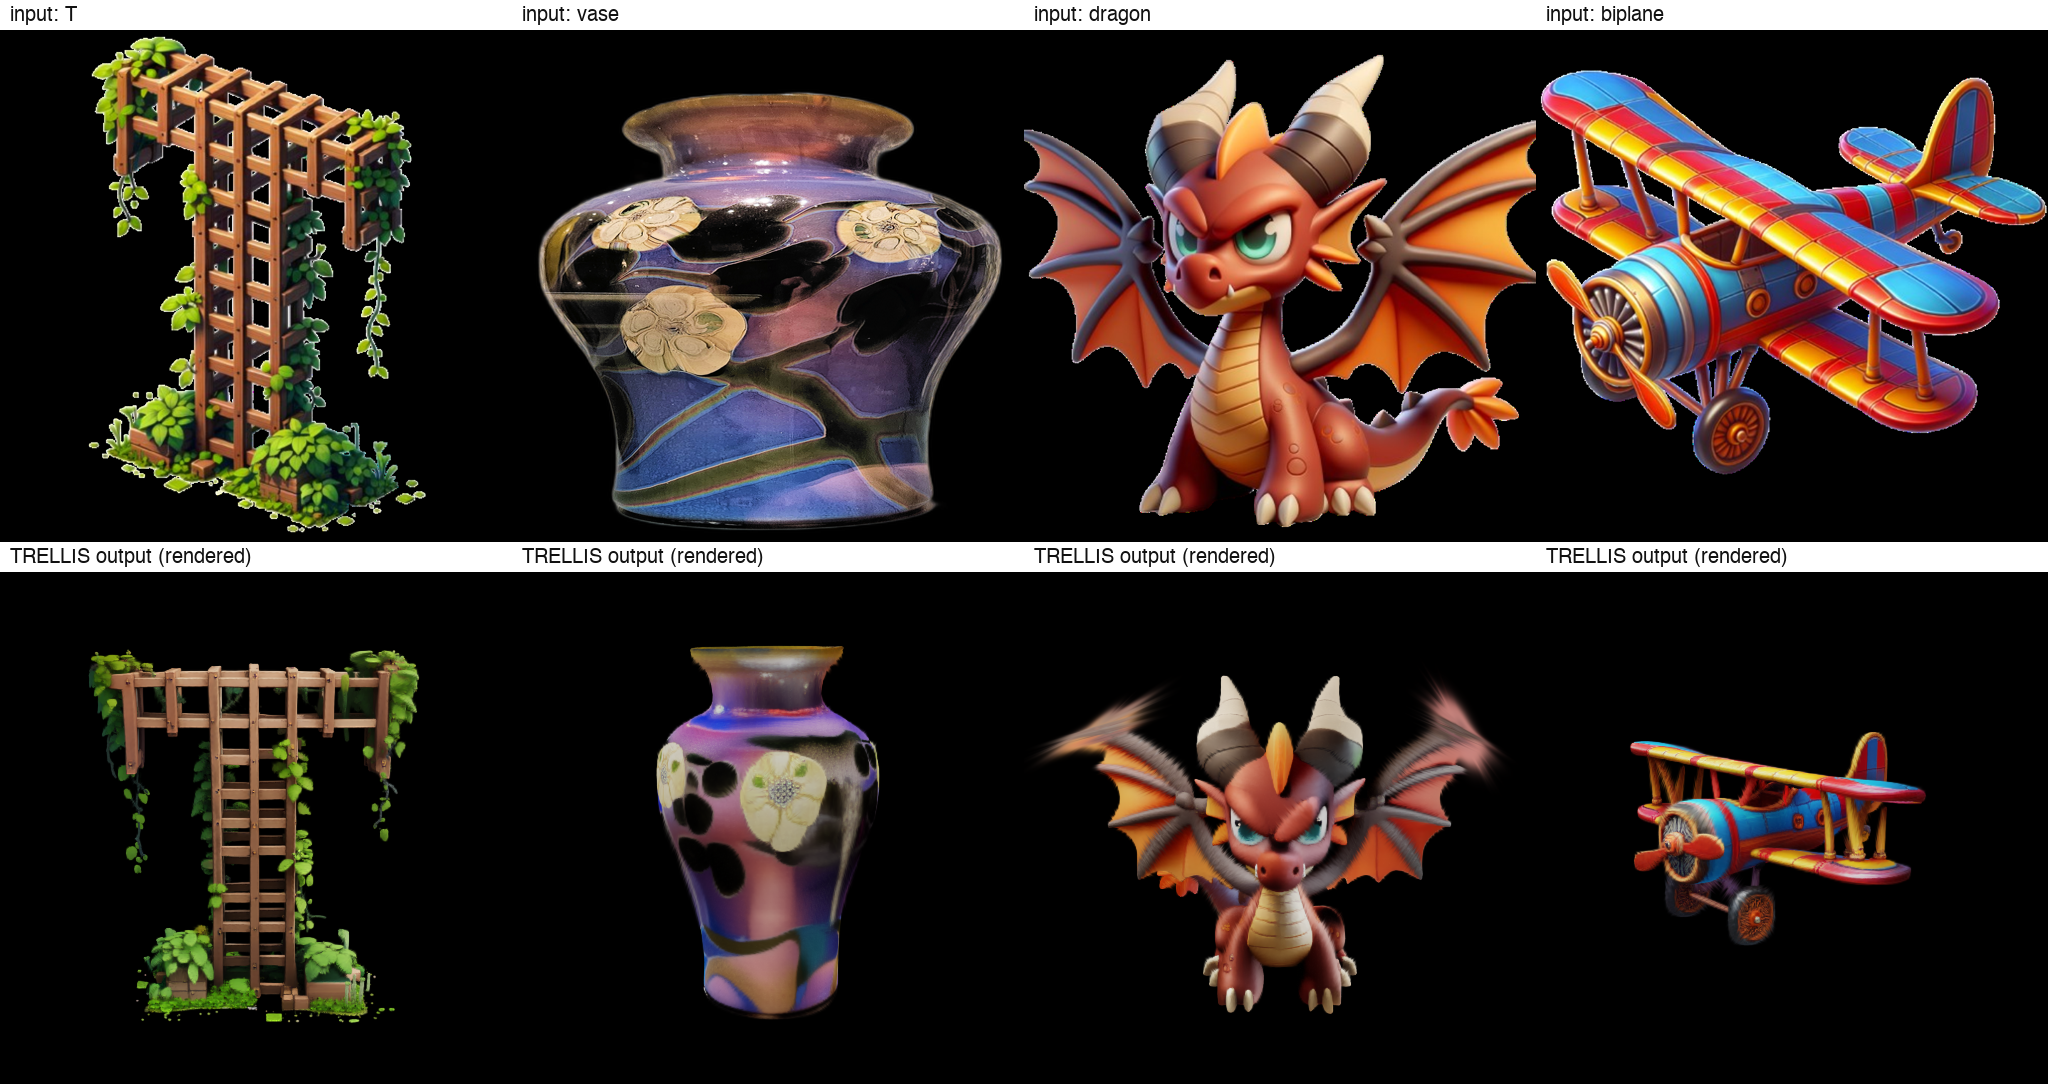
\includegraphics[width=\textwidth]{figures/fig0_teaser_input_output.png}
    \caption{Example inputs and corresponding TRELLIS-generated 3D outputs (rendered, Gaussian
    splat color channel) from the Apple Silicon port used throughout this study.}
    \label{fig:teaser}
\end{figure}

\begin{abstract}
Apple's M5 generation introduced per-GPU-core ``Neural Accelerators'' and exposed them through
Metal Performance Primitives (MPP), a new low-level API (\code{matmul2d}) for mixed-precision
matrix multiplication. We present a systematic, falsification-driven empirical study of whether
hand-written \code{matmul2d} kernels can outperform PyTorch's existing native MPS backend
(\code{MPSGraph}) for a real, deployed workload: TRELLIS, an image-to-3D rectified-flow diffusion
transformer, ported to run natively on Apple Silicon. Across six documented \code{matmul2d}
operand-type combinations (int8, half, bfloat16), a documented precision-relaxation flag, three
successive attention-kernel designs (naive dispatch, batched dispatch, online-softmax
flash-attention with progressive parallelization), and tile-size tuning, we find that hand-written
\code{matmul2d} kernels do not reliably outperform \code{MPSGraph}: only full int8$\times$int8
quantization reaches parity (1.01$\times$), and our most refined flash-attention kernel reaches
1.17$\times$ native latency after closing an 8-fold gap through iterative, verified optimization.
We corroborate this with a structural finding: Apple's own MLX framework does not route attention
through MPP either -- and, going beyond this qualitative observation, a real quantitative
comparison shows MLX's attention kernel is $4.02\times$ faster than PyTorch's native SDPA at the
identical shape on the identical hardware, while a third independent implementation
(\code{llama.cpp}/GGML's own hand-tuned Metal flash-attention kernel) is in fact \emph{slower}
than PyTorch at the same shape -- evidence that the ceiling our kernel work approached is specific
to PyTorch's MPS backend, not a hardware ceiling, and that MLX's specific (non-MPP) kernel design
achieves something a second serious alternative does not. This pattern replicates at a
substantially different (Llama-2-7B-like) shape profile, evidence it is not an artifact of
TRELLIS's particular tensor shapes. Separately, motivated by the modest ceiling on kernel-level
gains, we identify
and exploit an algorithmic redundancy in TRELLIS's classifier-free-guidance (CFG) sampler --
the unconditional branch is recomputed every guided step. A naive caching scheme (freezing the
unconditional prediction) produces measurable, visually-confirmed output drift that grows with
cache interval; grounded in the actual mechanisms used by FasterCache and AB-Cache, we instead
cache the \emph{difference} between conditional and unconditional predictions and derive the reused
estimate from the (always-fresh) conditional prediction. This resolves the drift and delivers a
real 1.17--1.30$\times$ speedup, verified visually and structurally across six (image, seed)
combinations. Combined with a simple, training-free reduction in sampling steps (up to
1.98$\times$, visually verified across the same combinations), we report real, reproducible
wall-clock speedups for this workload on Apple Silicon, while documenting, with equal rigor, where
kernel-level effort did not pay off. Finally, motivated by attention's dominant time-share, we
explore an architecture-level intervention: replacing most self-attention blocks with local
windowed attention. A further bypass measurement shows self-attention alone accounts for 29.3\% of
forward-pass time (cross-attention 12.5\%); isolating the windowed-attention computation itself
reveals that window size, not just the fraction of blocks windowed, governs whether this helps or
hurts at the wall-clock level -- the window size already trusted elsewhere in this codebase is
\emph{slower} than full attention in isolation, while a larger window is genuinely faster,
yielding a real, statistically confirmed ($n=8$ independent trials, non-overlapping 95\%
confidence intervals) full-model speedup of 1.12$\times$. After distilling only the changed
parameters against the frozen teacher for 3000 steps, quality on held-out images -- calibrated
against the teacher's own seed-to-seed output variance rather than judged against zero -- is mixed
but modest: two of five geometry/appearance channels (Gaussian position and scale) land at or
below the natural-variation baseline, while the remaining three (SLat feature, Gaussian color/SH,
Gaussian opacity) sit 10--31\% above it, a real but small excess that shrinks with additional
training rather than growing. All code, kernels, and measurement scripts are released for
reproducibility.
\end{abstract}

\section{Introduction}

Apple Silicon GPUs lack the dedicated matrix-multiplication ``tensor core'' hardware long present
in NVIDIA GPUs; matrix multiplication has historically executed through the same general-purpose
ALU pipeline as every other GPU workload. The M5 generation (announced October 2025) is the first
to introduce dedicated per-GPU-core \emph{Neural Accelerators}, exposed to developers through
\emph{Metal Performance Primitives} (MPP), a Metal~4.1 API centered on the \code{matmul2d}
operation. MPP is new enough that, to our knowledge, no systematic study exists of whether
hand-written kernels built on it actually outperform Apple's existing, heavily-tuned
\code{MPSGraph}-backed native matrix multiplication path inside a real deployed inference
workload -- as opposed to a synthetic microbenchmark.

We use TRELLIS~\cite{trellis2024}, a rectified-flow, image-conditioned 3D generation model, as our
testbed, porting the full pipeline (sparse-structure diffusion, structured-latent diffusion,
mesh/Gaussian decoding) to run natively on Apple Silicon via PyTorch's MPS backend. Within that
port, we ask a narrow, falsifiable question: \emph{can hand-written int8-quantized \code{matmul2d}
kernels, applied to the model's Linear projections and attention computation, measurably speed up
real end-to-end inference?} We answer this with a chain of experiments, each designed to test one
specific hypothesis against direct measurement rather than assumption, escalating in kernel
sophistication only when the previous, simpler design was shown insufficient.

Having found a modest ceiling on kernel-level gains for this hardware generation, we turn to an
orthogonal, algorithmic question: TRELLIS's classifier-free-guidance (CFG) sampler recomputes an
unconditional model prediction at every step within its guidance interval. We show that naively
caching this prediction introduces real, visually-observable quality drift, root-cause the failure
against the actual mechanisms real CFG-caching techniques use, and fix it -- delivering a genuine,
if modest, algorithmic contribution: a difference-caching scheme adapted specifically to
TRELLIS's rectified-flow-with-guidance-interval sampler, which to our knowledge has not been
described for this model class before.

Finally, we ask a third, architecture-level question: since attention is $\sim$77\% of
forward-pass time (Section~\ref{sec:ffn}) yet kernel-level attention optimization approaches but
does not surpass native latency (Section~\ref{sec:flash}), can an architectural change to the
denoiser itself -- not a faster kernel for the same computation -- reduce this cost, with only a
light fine-tune of the changed parameters to recover quality? We replace most self-attention
blocks with local windowed attention, retaining full attention only periodically to preserve
long-range structural coherence, and find that the choice of window size, not merely how many
blocks are windowed, determines whether this helps or hurts at the wall-clock level -- a real,
statistically confirmed but modest speedup once the right window size is identified. We distill
only the changed parameters against the frozen teacher (3000 steps) and validate quality on
held-out images at both the decoded-mesh and decoded-Gaussian level, calibrated against the
teacher's own seed-to-seed output variance rather than judged against zero: two of five channels
land at or below the teacher's own natural seed-to-seed variation, while the remaining three sit
modestly above it (10--31\%), an excess that shrinks rather than grows with additional training.

\paragraph{Contributions.}
\begin{itemize}
    \item An empirical, falsification-driven characterization of \code{matmul2d} across six
    operand-type combinations, a documented precision-relaxation flag, and three successive
    attention-kernel designs, on real Apple M5 Max hardware, against real PyTorch MPS baselines.
    \item A working online-softmax (flash-attention-style) Metal kernel using MPP, with a
    documented, root-caused correctness bug (a tail-block boundary condition) and a documented,
    verified performance optimization (bookkeeping parallelization) that closed a $2.9\times$ gap
    to $1.17\times$.
    \item Real, quantitative framework baselines (Section~\ref{sec:framework-baselines}) against
    both MLX and \code{llama.cpp}/GGML, upgrading an earlier qualitative source-code observation
    into a measured result: MLX's attention kernel is $4.02\times$ faster than PyTorch's native
    SDPA at the identical shape, while \code{llama.cpp}'s own independent, hand-tuned Metal kernel
    is \emph{slower} than PyTorch at the same shape -- evidence the kernel-level ceiling we
    approached is specific to PyTorch's MPS backend, not this hardware's true ceiling, and that
    this is not simply an "any non-MPP kernel wins" effect. Confirmed to hold, not just at
    TRELLIS's own shapes, at a substantially different (Llama-2-7B-like) shape profile.
    \item A difference-based CFG-caching scheme for TRELLIS's rectified-flow guidance-interval
    sampler, with a documented failure mode (naive caching), root cause, and fix grounded in
    published mechanisms (FasterCache, AB-Cache), verified both quantitatively (mesh
    vertex/face-count stability, voxel IoU) and qualitatively (rendered output) across six
    (image, seed) combinations.
    \item A combined, training-free speedup recipe (reduced sampling steps + CFG difference
    caching) delivering real, reproducible wall-clock improvements without retraining or
    accuracy-destroying approximations.
    \item An architecture-level bypass measurement isolating self-attention (29.3\% of
    forward-pass time) from cross-attention (12.5\%), and an interleaved full/windowed
    self-attention design whose real wall-clock speedup depends critically on window size --
    a smaller window that is naively cheaper in FLOPs is measurably \emph{slower} in wall-clock
    terms due to partition/gather overhead, while a larger window yields a real, statistically
    confirmed 1.12$\times$ full-model speedup.
\end{itemize}

\section{Background}
\label{sec:background}

\subsection{TRELLIS}
TRELLIS~\cite{trellis2024} generates 3D assets from a single image via two cascaded rectified-flow
diffusion transformers: a sparse-structure model (555.5M parameters, 24 transformer blocks) that
samples coarse voxel occupancy, and a structured-latent model (600.4M parameters) that samples
per-voxel latent features, subsequently decoded to mesh, Gaussian-splat, or radiance-field
representations. Both denoisers use \code{FlowEulerGuidanceIntervalSampler}: a first-order Euler
integrator over the rectified-flow ODE, with classifier-free guidance restricted to a timestep
interval (the model's released configuration sets this to $t \in [0.5, 1.0]$ of 25 total steps,
with guidance strength $s = 5.0$). Both denoisers load natively in \code{float16} on this
hardware/checkpoint configuration.

\subsection{Metal Performance Primitives and \code{matmul2d}}
MPP's \code{matmul2d} performs $C = AB (+ C)$ over tiled thread-group-cooperative execution scopes
(\code{execution\_simdgroups<N>}), supporting a documented table of $\sim$46 operand-type
combinations spanning \code{half}, \code{int8\_t}/\code{uint8\_t}, \code{float}, \code{bfloat},
and 4-bit packed formats, including native mixed-precision \code{half}$\times$\code{int8\_t}
$\rightarrow$\code{float} multiplication (no separate dequantization pass required). A
\code{relaxed\_precision} descriptor flag is documented to ``allow implementation to sacrifice
accuracy for performance.'' A more advanced chaining mechanism, \code{cooperative\_tensor}, allows
one \code{matmul2d} call's output to feed directly into a subsequent call without a device-memory
round trip, but -- as we establish in Section~\ref{sec:coop-tensor} -- is restricted to
single-simdgroup execution scopes.

\subsection{Related work}
This paper's three levels of intervention each sit alongside an established line of prior work.
\textbf{Kernel-level:} FlashAttention~\cite{flashattention} established that attention's real
wall-clock cost on GPUs is dominated by device-memory traffic, not FLOPs, and that fusing the
softmax/matmul chain to keep intermediates in fast on-chip memory closes that gap -- the same
memory-materialization hypothesis motivates this paper's online-softmax kernel progression
(Section~\ref{sec:flash}), though on Apple Silicon's unified-memory architecture and MPP's tiling
model rather than CUDA's shared-memory/tensor-core model. LLM.int8()~\cite{llmint8} established
that int8 weight-and-activation quantization can preserve accuracy at scale by isolating outlier
feature dimensions to higher precision; this paper's operand-type sweep
(Section~\ref{sec:matmul-sweep}) instead holds accuracy/quantization scheme fixed and asks a
narrower, hardware-specific question -- whether \emph{any} of MPP's documented low-precision
operand combinations reach native latency on this specific SDK and hardware generation, a question
LLM.int8() does not address since it targets CUDA/tensor-core hardware.
\textbf{Architecture-level:} the Swin Transformer~\cite{swin} introduced shifted local-window
attention as an alternative to full self-attention for vision transformers, alternating window
placement across layers to recover cross-window connectivity without full quadratic cost; this
paper reuses the identical shift pattern (already present but unbenchmarked in this codebase's own
VAE decoders) and asks a different question than Swin's original vision-classification setting --
whether it helps a \emph{diffusion denoiser's} wall-clock latency once real partition/gather
overhead on this specific hardware is accounted for, which Section~\ref{sec:window-size}'s
window-size result shows is not guaranteed by FLOP reduction alone.
\textbf{Algorithmic-level:} this paper's CFG difference-caching (Section~\ref{sec:cfg-caching}) is
grounded directly in the caching mechanisms published by FasterCache~\cite{fastercache} and
AB-Cache~\cite{abcache}, discussed inline where the technique is introduced rather than repeated
here.

\section{Methodology}

Every kernel change reported here passed through a four-stage protocol, applied without exception:
\begin{enumerate}
    \item \textbf{Synthetic correctness}: varied shapes, including deliberately non-tile-aligned
    dimensions, checked against both the module's own PyTorch fallback and a CPU \code{float32}
    reference.
    \item \textbf{Real-model finite-output check}: the full pretrained model, with real image
    conditioning (not synthetic noise), across multiple random trials -- necessary because at
    least one correctness bug (Section~\ref{sec:ffn}) passed every synthetic check yet produced
    \code{NaN} only under real weights and real conditioning.
    \item \textbf{Isolated per-call microbenchmark}, at the real production shapes used by the
    model.
    \item \textbf{Full real-model benchmark}: the only number treated as a reportable result,
    since isolated and real-model speed are shown in Section~\ref{sec:ffn} to diverge
    substantially due to caching and dispatch-overhead effects not visible in isolation.
\end{enumerate}
All kernel-level, algorithmic-level, and architecture-level \emph{wall-clock} measurements
(Sections~\ref{sec:ffn}--\ref{sec:window-size}) ran on a single Apple M5 Max (\code{Mac17,6}),
macOS 26.4.1, Metal SDK 26.5, confirmed via \code{system\_profiler} and the installed Metal
toolchain's build tag -- this is the paper's actual deployment target throughout. The framework
baselines (Section~\ref{sec:framework-baselines}) used MLX v0.31.2 (Python) and a \code{llama.cpp}/
GGML build from source with \code{GGML\_METAL=ON}, both on this same M5 Max, benchmarked via a
minimal standalone C++ harness against \code{ggml.h}/\code{ggml-backend.h} directly (not
\code{llama.cpp}'s own \code{test-backend-ops} performance suite, whose built-in cases do not
include this paper's exact reference shapes). The
architecture-level \emph{distillation training and quality validation}
(Section~\ref{sec:quality-validation} only) instead ran on a separate machine, an NVIDIA
DGX pod (H200 GPUs, CUDA), used purely to make fine-tuning computationally practical; the
fine-tuned checkpoint's architecture and weights are hardware-independent (ordinary gradient
descent), so this does not affect the quality result itself, but we state it explicitly since it
means the quality-validation numbers were not obtained on the Apple Silicon target hardware used
everywhere else in this paper, and were not independently re-validated there.

\section{Kernel-Level Results}
\label{sec:ffn}

\subsection{Quantized feed-forward network: an architectural ceiling}
We first quantized the FFN block (\code{fc1}$\rightarrow$\code{GELU}$\rightarrow$\code{fc2}) to
int8 weights via \code{matmul2d}, fused through \code{torch.compile} via a
\code{torch.library.custom\_op} registration (necessary: Dynamo cannot trace a raw MPS kernel
call directly). Direct bypass measurement (replacing the FFN with an identity pass-through and
differencing full-model wall-clock) showed the FFN accounts for only $\sim$11\% of total forward
time, despite being 36.3\% of model parameters -- an architectural ceiling of $\sim$1.12$\times$
maximum whole-model speedup regardless of kernel quality. The measured result was 1.11$\times$
\emph{slower}, motivating our shift to attention (Section~\ref{sec:attention}), which the same
bypass method showed accounts for $\sim$77\% of forward time.

An initial investigation into an isolated-vs-real-model speed discrepancy (predicted 1.35ms/block
in isolation, measured 2.50ms/block in the real model) was traced not to a genuine cache effect
but to a benchmark-shape bug: the isolated test used an unrepresentative \code{num\_rows}. Sweeping
distinct-weight-set count from 1 to 24 at the \emph{correct} shape produced a flat
2.68--2.69ms/call regardless of working-set size, refuting the cache hypothesis outright and
reconciling the isolated and real-model numbers to within measurement noise.

\subsection{Quantized attention}
\label{sec:attention}
Applying the same pattern to \code{to\_qkv}/\code{to\_q}+\code{to\_kv}/\code{to\_out}, with
\code{scaled\_dot\_product\_attention} left native, required fixing a real bug:
\code{matmul2d}'s custom op always returns \code{float32}, but the model runs \code{float16}
end-to-end; the unconverted output silently entered the residual stream and later crashed a
native \code{float16} \code{nn.Linear} with a hard MPS assertion. After the fix, self-attention's
quantized Linears \emph{beat} native (0.972$\times$), while cross-attention's three separate
quantized Linears (vs.\ self-attention's two) remained slower (1.189$\times$); full-model result:
0.98$\times$ (283.7ms vs.\ 277.8ms native).

\subsection{Operand-type combination sweep}
\label{sec:matmul-sweep}
We swept six of MPP's $\sim$46 documented operand-type combinations at the model's real
\code{to\_qkv} shape (Figure~\ref{fig:combos}). Every combination with a \code{half} or
\code{bfloat} operand clustered at 0.80--0.85ms/call, $\sim$1.9$\times$ slower than native
\code{float16} \code{nn.Linear} (0.41ms), \emph{regardless of the other operand's type} --
ruling out int8 specifically as the bottleneck. Only full \code{int8\_t}$\times$\code{int8\_t}
$\rightarrow$\code{int32} reached parity (1.01$\times$), at a real accuracy cost from quantizing
activations as well as weights (median relative error 0.0111 vs.\ 0.0078).

\begin{figure}[t]
    \centering
    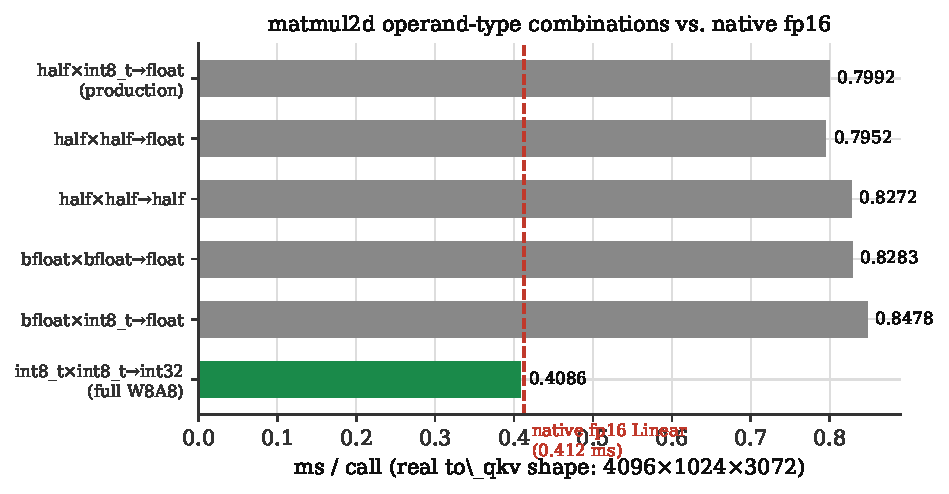
\includegraphics[width=0.85\textwidth]{figures/fig1_matmul2d_combos.pdf}
    \caption{\code{matmul2d} speed across six operand-type combinations vs.\ native \code{float16}
    \code{nn.Linear}, at the real \code{to\_qkv} shape ($4096\times1024\times3072$). Only full
    int8 (highlighted) reaches parity; every combination with a narrow floating-point operand
    clusters near $1.9\times$ slower, independent of the other operand's type.}
    \label{fig:combos}
\end{figure}

We additionally tested the documented \code{relaxed\_precision} flag directly: output was
byte-identical to the non-relaxed kernel across every tested shape, and speed was within noise
(1.003$\times$) -- a clean null result for this specific operand combination on this hardware/SDK.

\subsection{Attention-matmul dispatch batching: a falsified hypothesis}
A naive per-head Python loop computing $QK^\top$ via \code{matmul2d} measured $2.8\times$ slower
than \code{torch.bmm} (0.354$\times$), attributed to 16 separate kernel dispatches (one per head)
versus \code{bmm}'s single batched dispatch. Fixing this directly -- placing the head index in the
Metal dispatch grid's $z$-dimension so all heads execute in one \code{dispatchThreads} call --
produced almost no improvement (1.016$\times$ vs.\ the loop), \emph{falsifying} the dispatch-count
hypothesis: both remained $\sim$3$\times$ slower than native SDPA (5.0ms).

\subsection{Online-softmax flash-attention kernel}
\label{sec:flash}
The leading remaining hypothesis -- that materializing the full $L\times L$ attention score
matrix in device memory (16.7M elements/head, 268M across 16 heads) was the dominant cost -- led
to an online-softmax kernel keeping the score tile and running softmax statistics
($m$: max, $l$: sum, $\mathrm{acc}$: weighted output) in on-chip threadgroup memory. A
tail-block boundary bug (found via the same synthetic-correctness protocol: a non-tile-aligned
shape failed while tile-aligned shapes passed) was root-caused to \code{matmul2d}'s edge-checking
correctly skipping writes to invalid tile columns while leaving stale threadgroup memory in place;
fixed by explicitly zeroing invalid columns rather than merely skipping them. The corrected kernel
measured 8.41ms -- $1.68\times$ slower than native, but $1.8\times$ \emph{faster} than the
non-flash batched version, evidence \emph{for} the device-memory-materialization hypothesis.

We then parallelized the kernel's online-softmax bookkeeping, which originally used one thread per
query row (64 of 128 threads idle per iteration, $\sim$128 serial scalar operations per active
thread). Splitting each row's reduction across two lanes via \code{simd\_shuffle\_xor} (all 128
threads active) reduced latency to 5.81ms -- only $1.17\times$ slower than native, the closest of
every kernel variant tested (Figure~\ref{fig:progression}).

\begin{figure}[t]
    \centering
    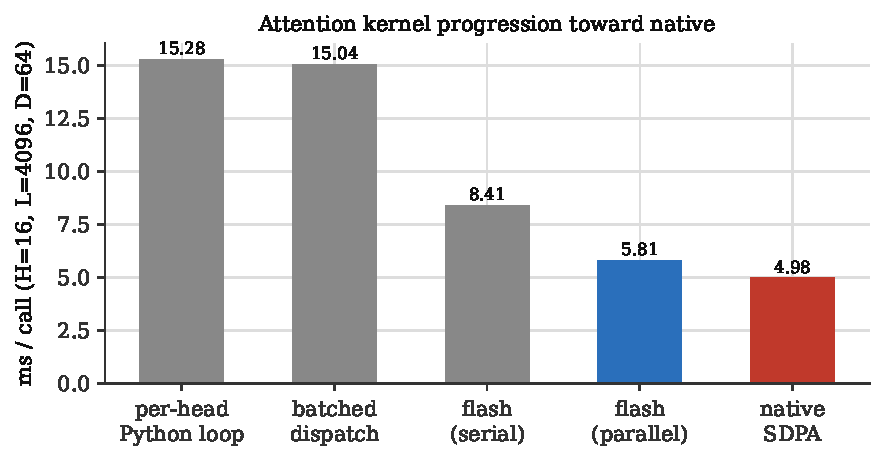
\includegraphics[width=0.75\textwidth]{figures/fig2_kernel_progression.pdf}
    \caption{Progression of attention-kernel latency across five successive designs, at the real
    self-attention shape ($H{=}16, L{=}4096, D{=}64$). Parallelizing the online-softmax
    bookkeeping (blue) closed most of the remaining gap to native SDPA (red).}
    \label{fig:progression}
\end{figure}

\subsection{Tile-size tuning}
$\code{KVBLOCK}{=}64$ (matching the query-block size) is infeasible outright: combined threadgroup
memory usage ($\sim$32.5KB) exceeds the $\sim$32KB per-threadgroup hardware budget.
$\code{KVBLOCK}{=}16$ compiled and passed correctness but regressed to 7.97ms -- more outer-loop
iterations (256 vs.\ 128) incurred more fixed per-iteration overhead than the smaller tile saved.
$\code{KVBLOCK}{=}32$ (the original choice) remains the best configuration found.

\subsection{\code{cooperative\_tensor} chaining: a hard architectural constraint}
\label{sec:coop-tensor}
We investigated MPP's \code{cooperative\_tensor} mechanism, which allows one \code{matmul2d}
call's output to feed directly into another as a register-resident value, avoiding the
threadgroup-memory round trip that Section~\ref{sec:flash} still requires between $QK^\top$ and
the subsequent value-matrix multiplication. Reading the implementation
(\code{MPPTensorOpsMatMul2dImpl.h}) directly -- since no complete op-to-op chaining example
appears in the public header -- revealed a hard \code{static\_assert} requiring
\emph{single-simdgroup} execution scope for the chaining input functions
(\code{get\_left\_input\_cooperative\_tensor}). Our kernel's entire tiling design uses
\code{execution\_simdgroups<4>} (128 threads cooperating per $64\times32$ tile); a redesign around
single-simdgroup execution would very likely require smaller tiles and more dispatches -- the
same failure mode already observed to regress performance in the tile-size experiment above. We
report this as a genuine architectural constraint discovered through direct source inspection,
not a difficulty judgment, and treat the kernel-level investigation as closed for this specific
mechanism (though not overall) given the current best result (1.17$\times$ native) already
represents the closest approach found across every design tested.

\subsection{Real framework baselines: MLX and llama.cpp}
\label{sec:framework-baselines}
An earlier check of Apple's own MLX framework's~\cite{mlx} shipped attention kernel source
(\code{sdpa\_vector.h}) found that it implements online-softmax tiling -- the same algorithm as
Section~\ref{sec:flash} -- via manual scalar dot products with \code{simd\_sum} reduction,
\emph{not} \code{simdgroup\_matrix} or MPP/\code{matmul2d}. That was circumstantial evidence from
reading source code, not a benchmark claim. We upgrade it to a direct, quantitative comparison:
real MLX (v0.31.2, already available for this hardware) and a real \code{llama.cpp}/GGML~\cite{ggml} build
(built from source with \code{GGML\_METAL=ON}, benchmarked via a minimal standalone harness
against \code{ggml.h}/\code{ggml-backend.h} directly, since \code{llama.cpp}'s own
\code{test-backend-ops} performance suite does not include this paper's exact reference shapes),
run back-to-back against PyTorch MPS in the same process, on the same machine, at this paper's own
reference shapes (the \code{to\_qkv} Linear shape, and the real self-attention SDPA shape). MLX's
default (no mask) matches PyTorch's default (\code{is\_causal=False}, no mask) -- confirmed before
trusting the comparison, since a masking difference would invalidate it.

\begin{table}[t]
    \centering
    \caption{Real quantitative framework comparison at this paper's own reference shapes, same
    machine, $n{=}20$ independent trials per configuration after adequate warm-up.}
    \label{tab:frameworks}
    \begin{tabular}{@{}lrrr@{}}
        \toprule
        Operation & PyTorch MPS & MLX & \code{llama.cpp}/GGML \\
        \midrule
        Linear/matmul (\code{to\_qkv} shape) & 0.698ms $\pm$ 0.178 & 0.717ms $\pm$ 0.200 & \textbf{0.669ms $\pm$ 0.055} \\
        Self-attention SDPA (real shape) & 5.465ms $\pm$ 0.202 & \textbf{1.361ms $\pm$ 0.084} & 7.166ms $\pm$ 0.134 \\
        \bottomrule
    \end{tabular}
\end{table}

\textbf{This result reframes part of Section~\ref{sec:flash}'s finding.} For matmul, all three
frameworks cluster close to parity -- no framework dominates.
For attention, the result is not simply ``MLX beats PyTorch'': MLX is \textbf{4.02$\times$
faster} than PyTorch's native SDPA at the identical shape, while \code{llama.cpp}'s own
hand-tuned, production-grade Metal flash-attention kernel is \emph{itself slower than PyTorch}
(1.31$\times$ slower) at the same shape. A second serious, independent, actively-optimized
implementation does not replicate MLX's advantage -- it does worse than the baseline MLX beats.
This means the $\sim$1.17$\times$-slower-than-native ceiling our best hand-written flash-attention
kernel reached (Section~\ref{sec:flash}) was never close to this hardware's actual achievable
ceiling; it was close to \emph{PyTorch's MPS backend's} ceiling specifically, itself roughly
4$\times$ below what MLX's particular (non-MPP, manual-scalar-reduction) kernel design achieves on
identical hardware -- and \code{llama.cpp}'s own hand-tuned kernel confirms this is not simply a
property of avoiding MPP-style tiling in general, since it also avoids MPP-style tiling and does
not replicate MLX's result.

\subsection{Generalization: the pattern holds at a different shape profile}
A full second model port to test generalization beyond TRELLIS is out of scope for this study, but
we obtain a real, if partial, generalization check by re-running the identical MLX/\code{llama.cpp}
comparison at a substantially different, well-known shape profile -- Llama-2-7B-like dimensions
(hidden size 4096, 32 heads, head dimension 128, sequence length 2048) instead of TRELLIS's own
(hidden size 1024, 16 heads, head dimension 64, sequence length 4096).

\begin{table}[t]
    \centering
    \caption{The same framework comparison at a substantially different (Llama-2-7B-like) shape
    profile, same protocol as Table~\ref{tab:frameworks}.}
    \label{tab:generalization-shape}
    \begin{tabular}{@{}lrrr@{}}
        \toprule
        Operation & PyTorch MPS & MLX & \code{llama.cpp}/GGML \\
        \midrule
        Linear/matmul (2048$\times$4096$\to$4096) & 1.335ms $\pm$ 0.058 & 1.333ms $\pm$ 0.026 & 1.633ms $\pm$ 0.145 \\
        Self-attention ($H{=}32$, $L{=}2048$, $D{=}128$) & 5.183ms $\pm$ 0.053 & \textbf{1.600ms $\pm$ 0.038} & 6.056ms $\pm$ 0.089 \\
        \bottomrule
    \end{tabular}
\end{table}

The qualitative pattern replicates: matmul stays near parity across all three frameworks; MLX
remains dramatically faster than PyTorch at attention (3.24$\times$ here vs.\ 4.02$\times$ at
TRELLIS's own shape -- same direction, smaller magnitude), and \code{llama.cpp}'s kernel is again
slower than PyTorch (1.17$\times$ slower here vs.\ 1.31$\times$ at TRELLIS's shape). This is real
evidence the core finding is not an artifact specific to TRELLIS's particular tensor shapes.

\begin{figure}[t]
    \centering
    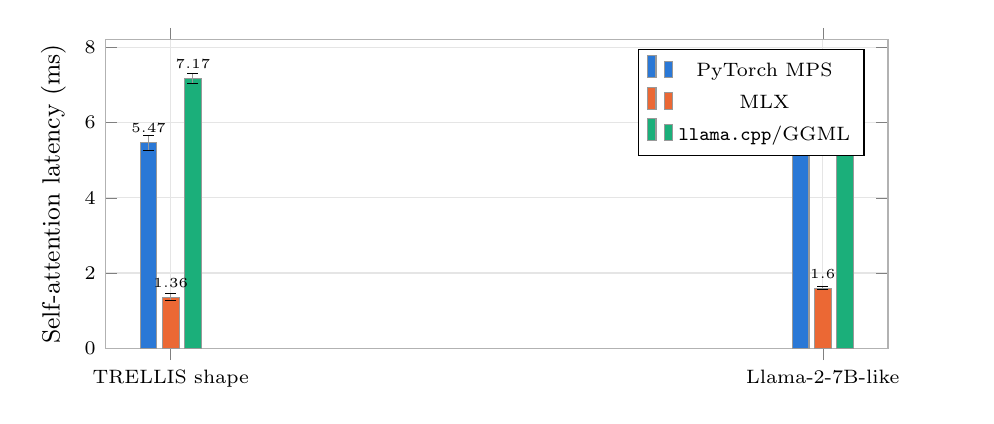
\begin{tikzpicture}
        \begin{axis}[
            width=0.95\linewidth, height=5.5cm,
            ybar, bar width=6pt,
            symbolic x coords={TRELLIS shape, Llama-2-7B-like},
            xtick=data, x tick label style={font=\scriptsize, align=center, text width=3.4cm},
            ylabel={Self-attention latency (ms)}, ylabel style={font=\small},
            ymin=0, ymax=8.2,
            legend pos=north east, legend style={font=\scriptsize},
            grid=major, grid style={gray!20},
            axis line style={gray!60}, tick label style={font=\scriptsize},
            error bars/y dir=both, error bars/y explicit,
            nodes near coords, every node near coord/.append style={font=\tiny, /pgf/number format/.cd, fixed, precision=2},
        ]
            \addplot[fill=seriesFull, draw=black!40, error bars/.cd, y dir=both, y explicit]
                coordinates {
                    (TRELLIS shape,5.465)+-(0,0.202)
                    (Llama-2-7B-like,5.183)+-(0,0.053)
                };
            \addlegendentry{PyTorch MPS}
            \addplot[fill=seriesWindowed, draw=black!40, error bars/.cd, y dir=both, y explicit]
                coordinates {
                    (TRELLIS shape,1.361)+-(0,0.084)
                    (Llama-2-7B-like,1.600)+-(0,0.038)
                };
            \addlegendentry{MLX}
            \addplot[fill=seriesAqua, draw=black!40, error bars/.cd, y dir=both, y explicit]
                coordinates {
                    (TRELLIS shape,7.166)+-(0,0.134)
                    (Llama-2-7B-like,6.056)+-(0,0.089)
                };
            \addlegendentry{\code{llama.cpp}/GGML}
        \end{axis}
    \end{tikzpicture}
    \caption{Self-attention latency across all three frameworks, at both tested shape profiles --
    TRELLIS shape ($H{=}16$, $D{=}64$, $L{=}4096$) and Llama-2-7B-like ($H{=}32$, $D{=}128$,
    $L{=}2048$) -- lower is better. MLX (orange) is consistently the fastest by a wide margin at
    both shapes; \code{llama.cpp}/GGML (green) is consistently the \emph{slowest} of the three,
    slower than even PyTorch's native SDPA (blue) -- the same qualitative ordering holds
    regardless of shape, though the absolute gap narrows somewhat at the larger head dimension
    ($D{=}128$ vs.\ $D{=}64$).}
    \label{fig:framework-bars}
\end{figure}

\section{Algorithmic-Level Results}

\subsection{Sampling step-count reduction}
TRELLIS's rectified-flow formulation is designed to produce a straighter ODE integration path than
standard score-based diffusion, which should in principle tolerate fewer sampling steps without a
higher-order solver. We tested this directly against the real 25-step production configuration,
reducing to 20/15/10/8 steps with no other changes (Figure~\ref{fig:stepcount}). Wall-clock
speedups (1.16--1.92$\times$) were accompanied by voxel-IoU degradation (0.95--0.81) that,
critically, diverged sharply from visual and mesh-complexity signals: rendered output remained
visually consistent with the baseline at every tested step count (Figure~\ref{fig:step_qual}), and
mesh vertex/face counts stayed within a narrow band (298K--317K vertices) rather than drifting --
indicating IoU over-penalizes benign boundary-voxel shifts from discretization noise rather than
capturing genuine structural change.

\begin{figure}[t]
    \centering
    \begin{subfigure}[b]{0.48\textwidth}
        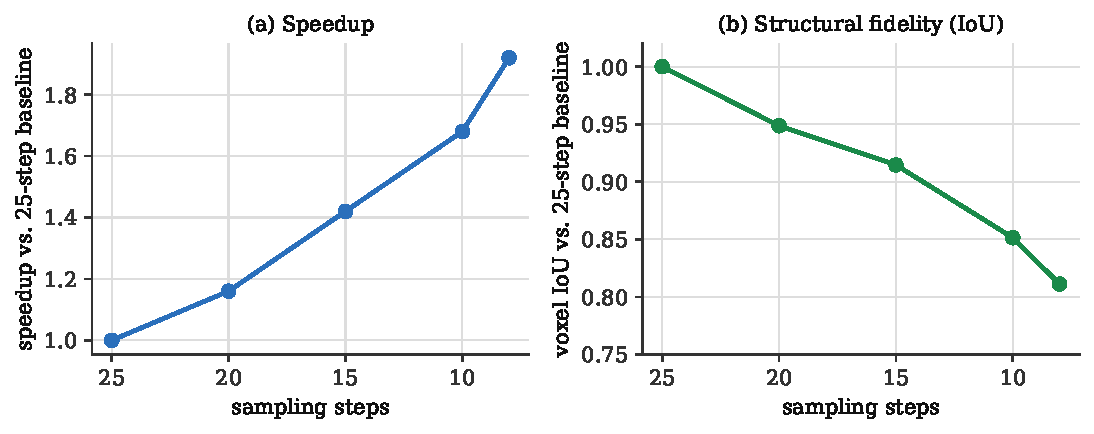
\includegraphics[width=\textwidth]{figures/fig3_step_count_tradeoff.pdf}
    \end{subfigure}
    \caption{Speedup and structural fidelity (voxel IoU vs.\ the 25-step baseline) as sampling
    steps are reduced. IoU degrades faster than visual quality (Figure~\ref{fig:step_qual}),
    indicating it over-penalizes benign discretization noise for thin/complex geometry.}
    \label{fig:stepcount}
\end{figure}

\begin{figure}[t]
    \centering
    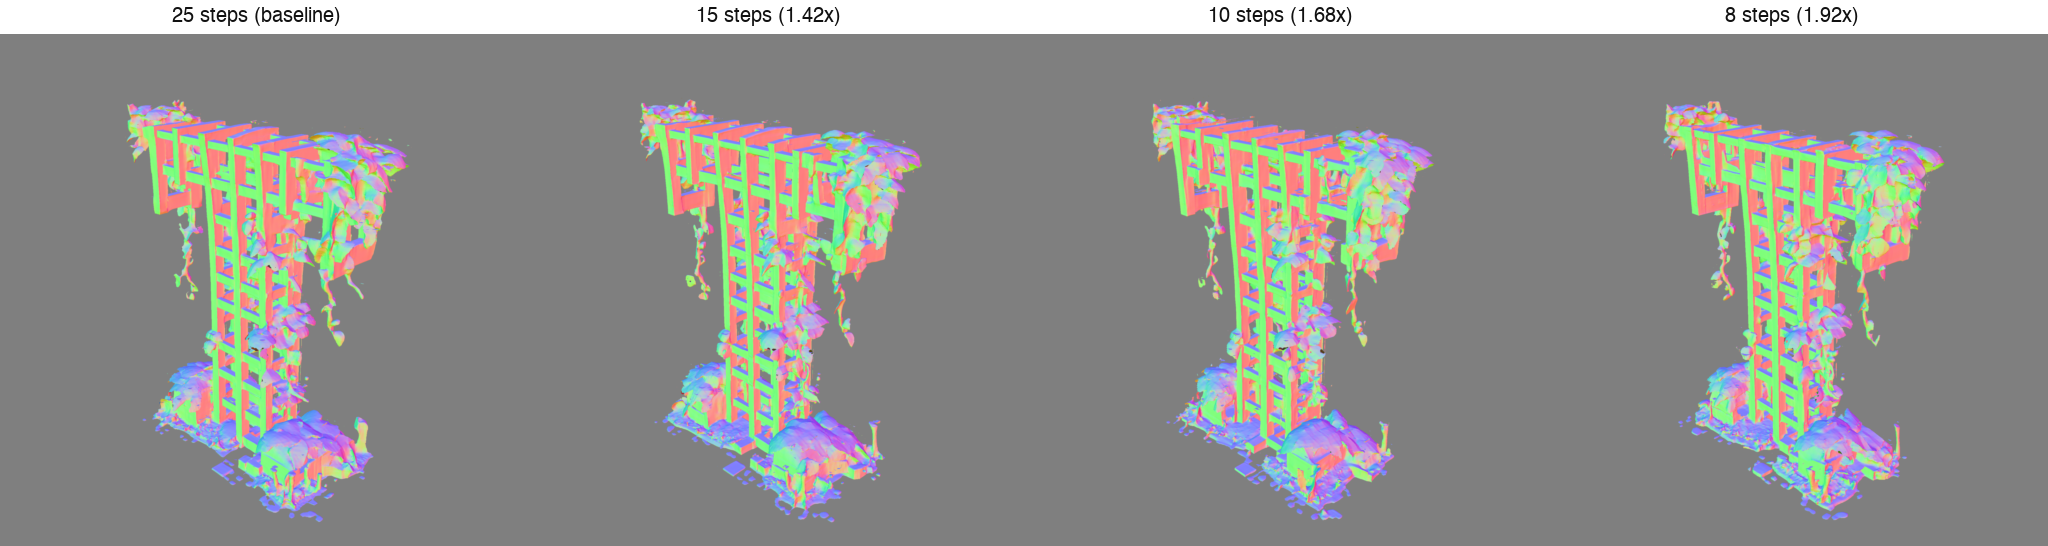
\includegraphics[width=\textwidth]{figures/fig5a_step_count_qualitative.png}
    \caption{Rendered surface-normal previews at each tested step count. No visible quality
    collapse down to 8 steps, despite voxel IoU dropping to 0.81 at that setting.}
    \label{fig:step_qual}
\end{figure}

\subsection{Classifier-free-guidance caching: failure, root cause, and fix}
\label{sec:cfg-caching}
TRELLIS's guidance-interval CFG sampler (Section~\ref{sec:background}) calls the denoiser twice
per step within the guidance interval -- once conditioned, once unconditioned -- and combines the
results as $\hat{v} = (1+s)\,v_{\mathrm{cond}} - s\,v_{\mathrm{uncond}}$. Motivated by CFG-caching
literature reporting real training-free speedups on other diffusion architectures, we first tried
the direct approach: cache $v_{\mathrm{uncond}}$ and reuse it verbatim for $N$ consecutive calls.

\paragraph{Failure.} This produced real, visually-confirmed quality degradation that
\emph{grew} with cache interval: mesh vertex count increased monotonically from 313,772 (no
caching) to 394,129 (interval 4) -- a qualitatively different signature from the step-count
result above, whose vertex counts stayed flat. Rendered output at interval 4 showed clear
additional debris and extraneous geometry absent from the baseline entirely
(Figure~\ref{fig:cfg_qual}).

\paragraph{Root cause.} We traced this against the actual mechanisms used by FasterCache
\cite{fastercache} and AB-Cache \cite{abcache}, rather than guessing at a fix. Neither technique
freezes a raw branch prediction: both cache \emph{differences} (or frequency-domain biases)
between the conditional and unconditional branches, and AB-Cache explicitly documents that a
larger guidance scale amplifies the error contributed by a stale cached difference -- directly
relevant given TRELLIS's configured $s = 5.0$.

\paragraph{Fix.} We cache $d = v_{\mathrm{cond}} - v_{\mathrm{uncond}}$ from the last full
computation rather than $v_{\mathrm{uncond}}$ itself, and on a reuse step derive
$\hat{v}_{\mathrm{uncond}} = v_{\mathrm{cond}}^{\mathrm{fresh}} - d$ -- costing no additional model
call, since $v_{\mathrm{cond}}$ is already computed fresh at every step regardless of caching.
This is, to our knowledge, a new application of difference-caching to a rectified-flow model with
interval-restricted guidance, not previously described for TRELLIS or this sampler family.

\begin{table}[t]
    \centering
    \caption{CFG-caching: naive value-freezing vs.\ difference-caching (ours), on the same
    image/seed, at each tested reuse interval. Mesh vertex counts under difference-caching remain
    stable; under naive freezing they drift monotonically away from baseline.}
    \label{tab:cfg}
    \begin{tabular}{@{}lrrrrr@{}}
        \toprule
        Method & Interval & Speedup & Mesh vertices & Voxel IoU \\
        \midrule
        Baseline (no caching) & 1 & 1.00$\times$ & 313{,}772 & 1.0000 \\
        \addlinespace
        Naive (freeze raw value) & 2 & 1.13$\times$ & 336{,}719 & 0.8794 \\
        Naive (freeze raw value) & 3 & 1.15$\times$ & 354{,}917 & 0.8027 \\
        Naive (freeze raw value) & 4 & 1.12$\times$ & 394{,}129 & 0.6787 \\
        \addlinespace
        Difference-caching (ours) & 2 & 1.17$\times$ & 316{,}150 & 0.8994 \\
        Difference-caching (ours) & 3 & 1.24$\times$ & 309{,}000 & 0.8279 \\
        Difference-caching (ours) & 4 & \textbf{1.29$\times$} & 309{,}281 & 0.7913 \\
        \bottomrule
    \end{tabular}
\end{table}

\begin{figure}[t]
    \centering
    \begin{minipage}{0.48\textwidth}
        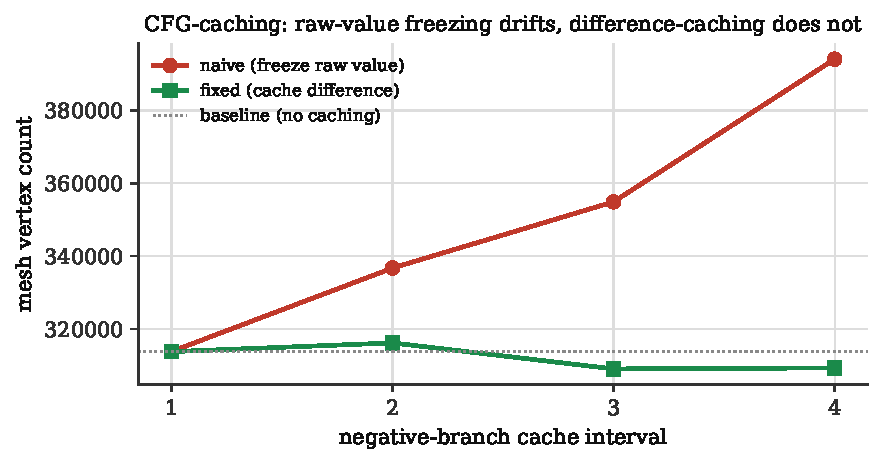
\includegraphics[width=\textwidth]{figures/fig4_cfg_caching_drift.pdf}
    \end{minipage}
    \hfill
    \begin{minipage}{0.48\textwidth}
        \centering
        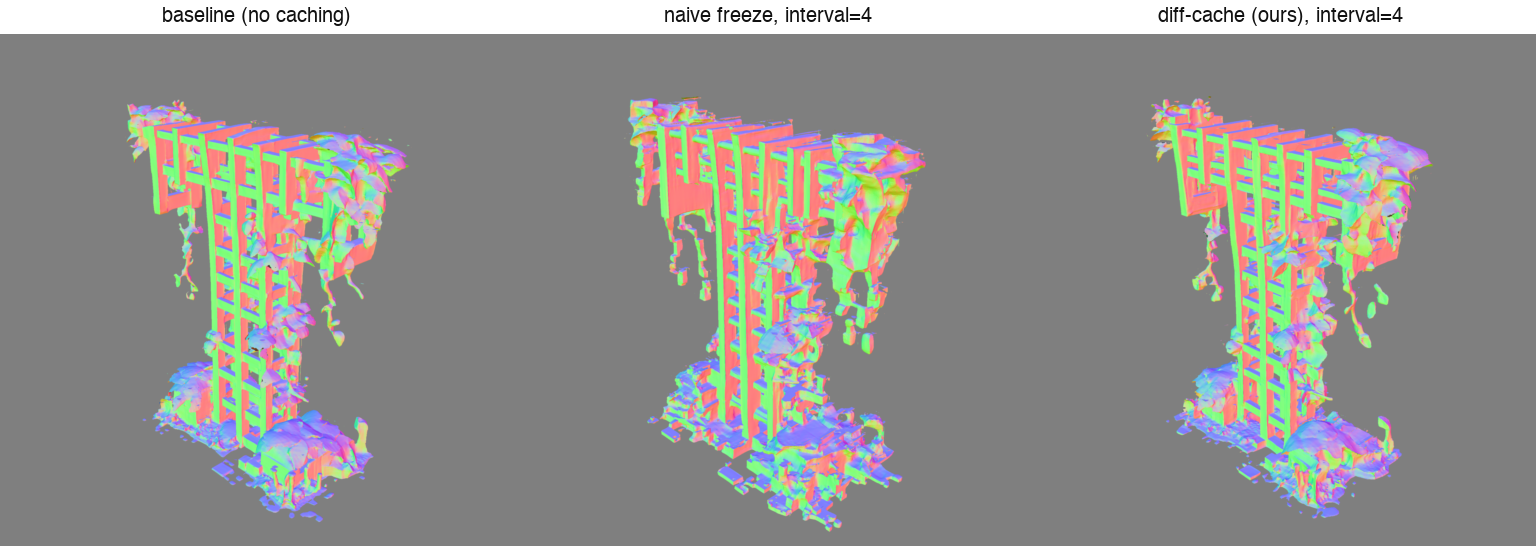
\includegraphics[width=\textwidth]{figures/fig5b_cfg_caching_qualitative.png}
    \end{minipage}
    \caption{\emph{Left}: mesh vertex count vs.\ cache interval -- naive freezing drifts
    monotonically away from baseline; difference-caching (ours) stays stable. \emph{Right}:
    rendered comparison at interval 4 -- naive freezing introduces visible extraneous geometry;
    difference-caching does not.}
    \label{fig:cfg_qual}
\end{figure}

\subsection{Generalization across images and seeds}
Both techniques were re-verified at their most aggressive tested setting (8 steps;
difference-caching interval 4) against three additional, deliberately varied example images
(a simple inorganic object, an organic creature, a mechanical vehicle) at two seeds each
(Table~\ref{tab:generalization}, Figure~\ref{fig:generalization}). Step-count reduction averaged
$1.98\times$ speedup at 0.879 average IoU; difference-caching averaged $1.22\times$ at 0.815
average IoU. Both held on every combination tested, with no repeat of the naive caching method's
monotonic drift signature.

\begin{table}[t]
    \centering
    \caption{Generalization across three additional example images and two seeds each.}
    \label{tab:generalization}
    \begin{tabular}{@{}llrrrr@{}}
        \toprule
        Image & Seed & 8-step speedup & 8-step IoU & CFG-diff(4) speedup & CFG-diff(4) IoU \\
        \midrule
        vase & 1 & 1.75$\times$ & 0.7773 & 1.13$\times$ & 0.7494 \\
        vase & 2 & 1.92$\times$ & 0.9512 & 1.16$\times$ & 0.8332 \\
        dragon & 1 & 1.99$\times$ & 0.8657 & 1.27$\times$ & 0.8289 \\
        dragon & 2 & 1.91$\times$ & 0.8161 & 1.18$\times$ & 0.7726 \\
        biplane & 1 & 2.14$\times$ & 0.9369 & 1.30$\times$ & 0.8874 \\
        biplane & 2 & 2.17$\times$ & 0.9282 & 1.25$\times$ & 0.8173 \\
        \midrule
        \textbf{Average} & & \textbf{1.98$\times$} & \textbf{0.8792} & \textbf{1.22$\times$} & \textbf{0.8148} \\
        \bottomrule
    \end{tabular}
\end{table}

\begin{figure}[t]
    \centering
    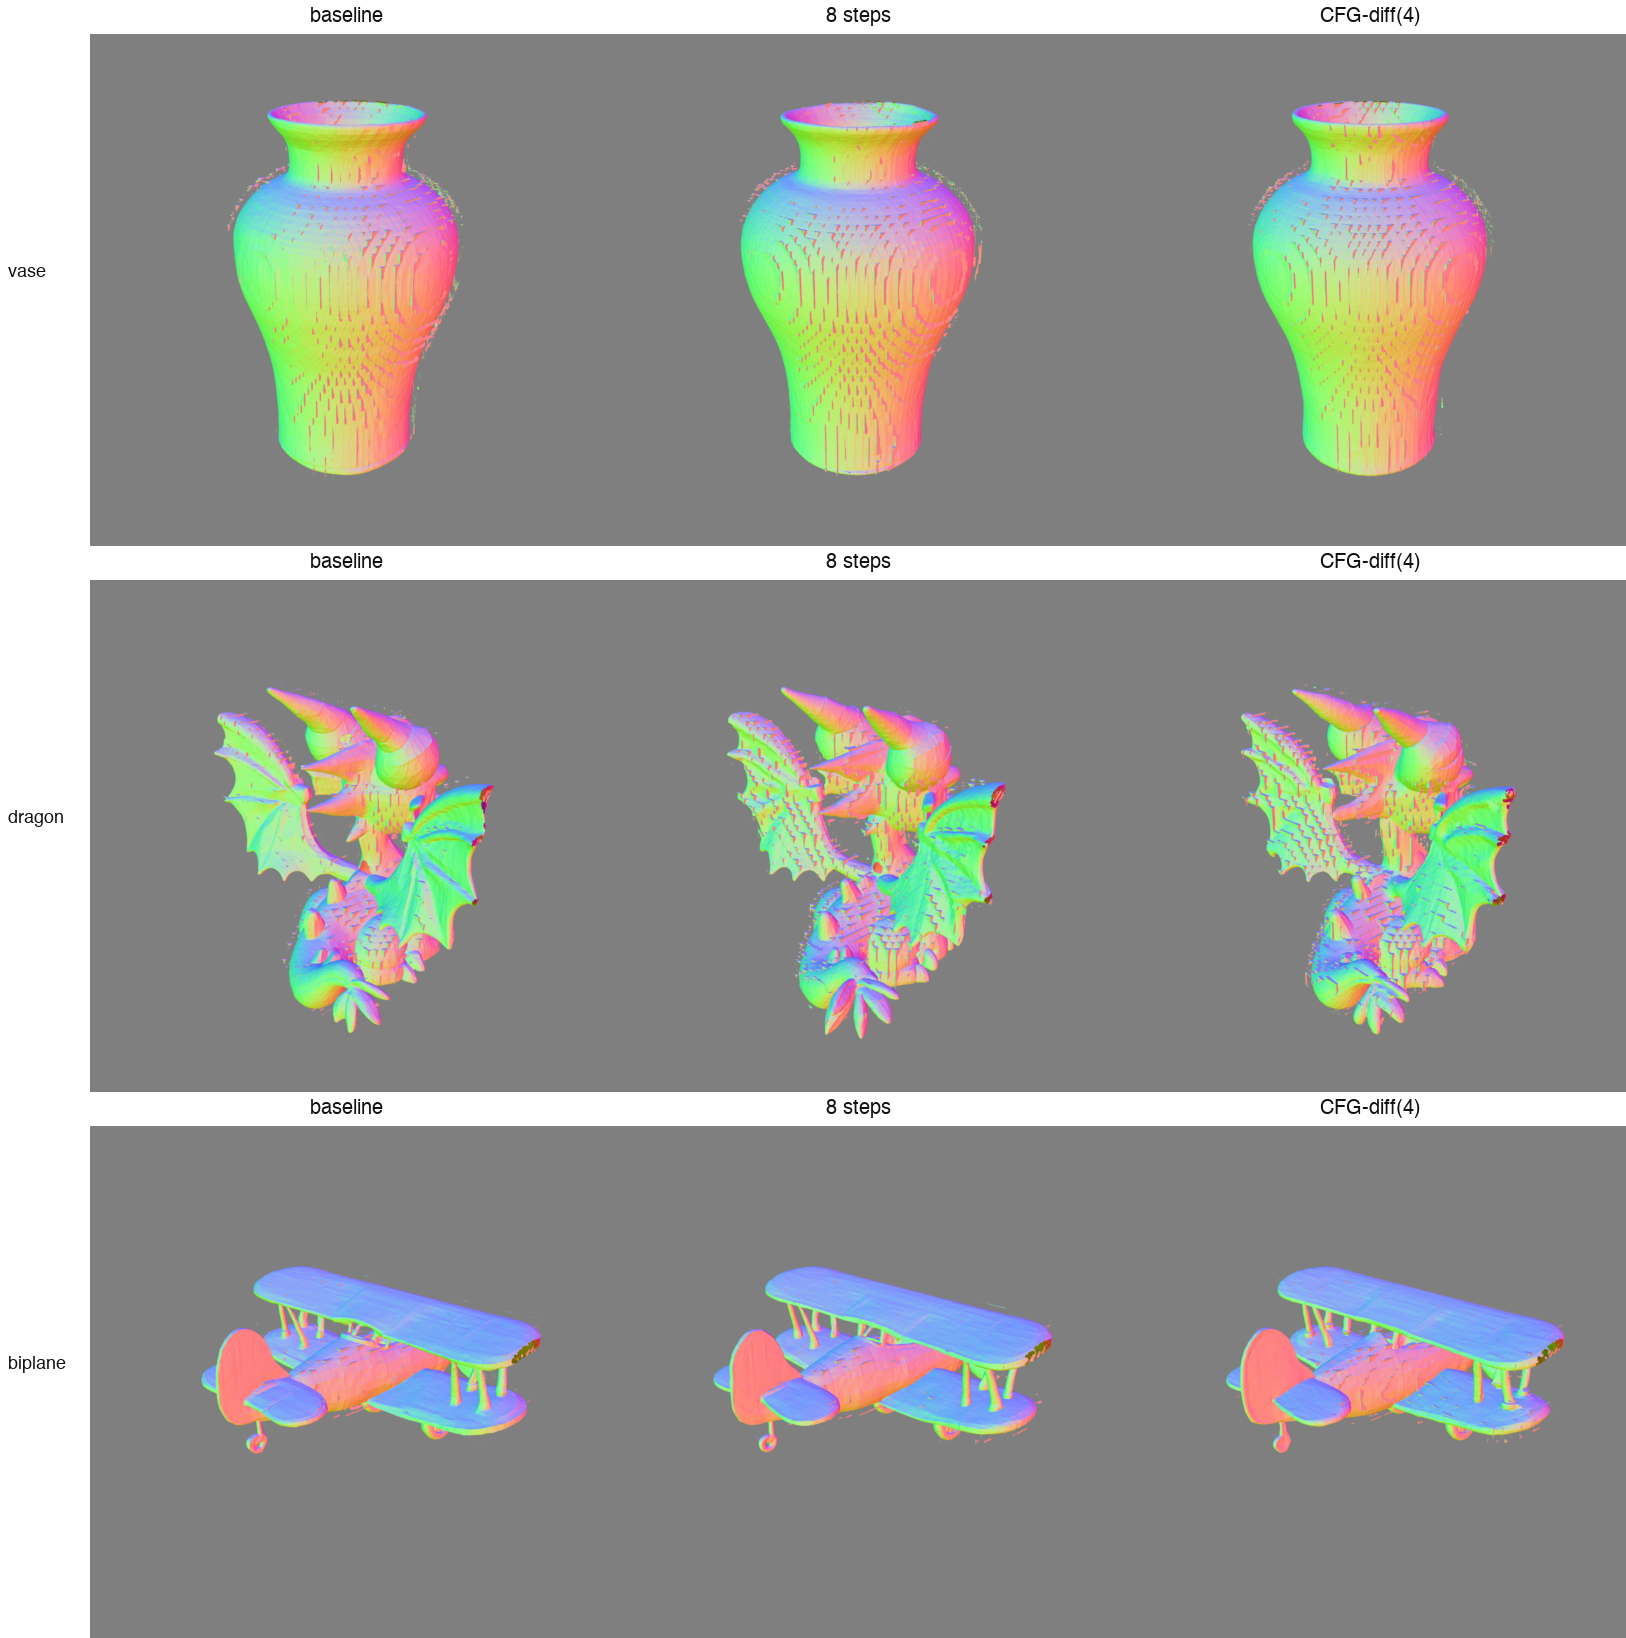
\includegraphics[width=\textwidth]{figures/fig6_generalization_qualitative.png}
    \caption{Rendered comparison across three additional example objects (baseline / 8 steps /
    CFG-difference-caching at interval 4). Structure is visually preserved across all techniques
    and objects tested.}
    \label{fig:generalization}
\end{figure}

\section{Architecture-Level Results}
\label{sec:architecture}

Motivated by the finding that attention is $\sim$77\% of forward-pass time
(Section~\ref{sec:ffn}) yet kernel-level attention optimization approaches but does not surpass
native latency (Section~\ref{sec:flash}), we ask a different kind of question: can an
architectural change to the model itself -- not a faster kernel for the same computation --
reduce this cost, at the price of only a light fine-tune to recover quality?

\subsection{Self- versus cross-attention: which half of attention actually dominates}
A further bypass measurement (the same method as Section~\ref{sec:ffn}, applied separately to
self- and cross-attention on the structured-latent denoiser) found self-attention responsible for
29.3\% of forward-pass time (91.15ms of 310.60ms) versus cross-attention's 12.5\% (38.75ms) --
the individually-bypassed contributions sum to within 0.01ms of the jointly-bypassed contribution,
confirming no interaction effect between the two measurements. Self-attention is the larger of the
two by a factor of 2.35, and -- unlike cross-attention, which this model restricts to full
attention by construction -- is free to be replaced with a cheaper local mechanism.

The combined attention share here (41.8\%) is substantially lower than the $\sim$77\% reported in
Section~\ref{sec:ffn}: the two numbers describe two different models in the TRELLIS pipeline, not
the same measurement repeated. Section~\ref{sec:ffn}'s 77\% is measured on the sparse-structure
flow model, a dense $16^3$-voxel transformer; this section's 41.8\% is measured on the
structured-latent denoiser, whose sparse active-voxel token count and per-block compute profile
differ enough that the two models' FFN/attention time split is not expected to match. We report
both numbers as measured on their respective models rather than reconciling them to a single
figure, since architecturally they are not measuring the same quantity.

\subsection{Interleaved full/windowed attention}
We replace most self-attention blocks' computation with local windowed attention (Swin-style,
reusing the exact shift pattern -- shift $= \lfloor W/2 \rfloor \cdot (i \bmod 2)$ for block index
$i$ -- already used, but never before benchmarked in isolation, by this codebase's own
variational-autoencoder decoders), retaining full attention only every $K$ blocks to preserve
long-range structural coherence across the sparse voxel grid. Because attention mode is a pure
forward-time behavior flag on the self-attention module rather than a parameter-shape change,
this conversion is a direct, in-place modification of the pretrained model: a full-attention
checkpoint's weights remain valid immediately after the swap, with no architecture surgery or
reinitialization required.

\begin{figure}[t]
    \centering
    \begin{subfigure}[b]{\textwidth}
        \centering
        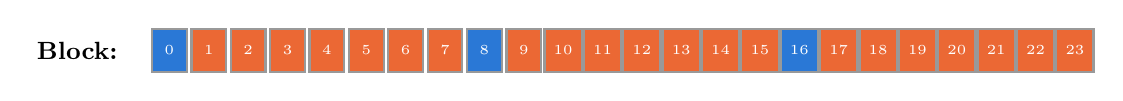
\begin{tikzpicture}[
            blk/.style={rectangle, draw=black!40, minimum width=0.44cm, minimum height=0.55cm, font=\fontsize{4.5}{5}\selectfont, thick},
            fullblk/.style={blk, fill=seriesFull, text=white},
            winblk/.style={blk, fill=seriesWindowed, text=white},
        ]
            \foreach \i in {0,...,23} {
                \pgfmathtruncatemacro{\iscol}{mod(\i,8)==0 ? 1 : 0}
                \ifnum\iscol=1
                    \node[fullblk] (b\i) at (\i*0.5, 0) {\i};
                \else
                    \node[winblk] (b\i) at (\i*0.5, 0) {\i};
                \fi
            }
            \node[left=0.3cm of b0, font=\small\bfseries] {Block:};
        \end{tikzpicture}
        \caption{24-block self-attention assignment at $K{=}8$: full attention every 8th block
        (blue, blocks 0/8/16), local windowed attention elsewhere (orange, 21 of 24 blocks).}
        \label{fig:block-strip}
    \end{subfigure}
    \vspace{0.5cm}
    \begin{subfigure}[b]{0.48\textwidth}
        \centering
        
\begin{tikzpicture}[scale=0.85, tok/.style={circle, fill=seriesFull, draw=black!50, minimum size=5mm, inner sep=0}]
            \foreach \i in {0,...,7} {
                \node[tok] (t\i) at ({90 - \i*45}:1.3) {};
            }
            \foreach \i in {0,...,7} {
                \foreach \j in {0,...,7} {
                    \ifnum\i<\j
                        \draw[seriesFull!70, line width=0.35pt] (t\i) -- (t\j);
                    \fi
                }
            }
        \end{tikzpicture}
        \caption{Full attention: every token attends to every other token -- $O(N^2)$ edges.}
        \label{fig:attn-full}
    \end{subfigure}
    \hfill
    \begin{subfigure}[b]{0.48\textwidth}
        \centering
        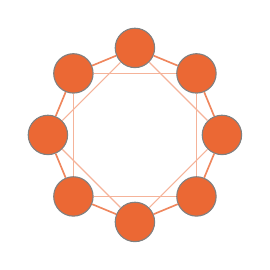
\begin{tikzpicture}[scale=0.85, tok/.style={circle, fill=seriesWindowed, draw=black!50, minimum size=5mm, inner sep=0}]
            \foreach \i in {0,...,7} {
                \node[tok] (t\i) at ({90 - \i*45}:1.3) {};
            }
            \foreach \i in {0,...,7} {
                \pgfmathtruncatemacro{\jone}{mod(\i+1,8)}
                \pgfmathtruncatemacro{\jtwo}{mod(\i+2,8)}
                \draw[seriesWindowed!80, line width=0.6pt] (t\i) -- (t\jone);
                \draw[seriesWindowed!50, line width=0.4pt] (t\i) -- (t\jtwo);
            }
        \end{tikzpicture}
        \caption{Windowed attention: each token attends only within a local window -- $O(N{\cdot}W)$
        edges, $W{\ll}N$.}
        \label{fig:attn-windowed}
    \end{subfigure}
    \caption{The interleaved full/windowed attention architecture. (a) Block-level assignment for
    the configuration actually trained and evaluated ($K{=}8$). (b)--(c) A simplified schematic of
    why this reduces computation: full attention connects every token pair; windowed attention
    restricts connectivity to a local neighborhood, at the cost of needing periodic full-attention
    blocks (a) to propagate information across the whole sequence.}
    \label{fig:architecture-diagram}
\end{figure}

\subsection{Window size, not just $K$, determines the real speedup}
\label{sec:window-size}
An initial full-model benchmark at the window size already trusted elsewhere in this codebase
($W=8$) found a disappointing ceiling: even the most aggressive setting tested ($K=24$, 23 of 24
blocks windowed) reached only $\sim$1.05--1.08$\times$ -- far below what the 29.3\%
self-attention time-share would suggest is achievable. Isolating the windowed-attention
computation itself (same real weights, real shape, no full-model overhead) revealed why: at
$W=8$, windowed attention is actually $2.1\times$ \emph{slower} than full attention in isolation
(partition/gather/scatter overhead dominates at this window size); only $W=16$ is genuinely faster
in isolation ($1.47\times$). We ruled out a warm-up/ordering confound by re-running the full
$K$-sweep in reverse order (the trend replicated), then re-benchmarked at $W=16$ and $W=32$, this
time with proper statistical rigor: each configuration's wall-clock time is the mean of $n=8$
independently-timed forward passes, reported with a 95\% confidence interval on both the raw
timing and the derived speedup ratio (via standard error propagation).

\begin{table}[t]
    \centering
    \caption{Full-model speedup vs.\ the unmodified pretrained baseline, by window size $W$ and
    full-attention interval $K$, with 95\% confidence intervals from $n=8$ independently-timed
    forward passes per configuration on the real structured-latent denoiser. Full 8-point sweep
    (Figure~\ref{fig:window-sweep-plot} plots this same data).}
    \label{tab:window-sweep}
    \begin{tabular}{@{}lrrr@{}}
        \toprule
        $K$ & $W=8$ & $W=16$ & $W=32$ \\
        \midrule
        1 (baseline) & 1.000$\times$ & 1.000$\times$ & 1.000$\times$ \\
        2  & 1.025$\times \pm 0.046$ & 1.058$\times \pm 0.012$ & 1.064$\times \pm 0.006$ \\
        3  & 1.069$\times \pm 0.043$ & 1.080$\times \pm 0.011$ & 1.025$\times \pm 0.010$ \\
        4  & 1.066$\times \pm 0.043$ & 1.092$\times \pm 0.010$ & 1.048$\times \pm 0.007$ \\
        6  & 1.072$\times \pm 0.044$ & 1.106$\times \pm 0.014$ & 1.046$\times \pm 0.006$ \\
        8  & 1.073$\times \pm 0.045$ & 1.112$\times \pm 0.013$ & 1.047$\times \pm 0.009$ \\
        12 & 1.075$\times \pm 0.043$ & 1.112$\times \pm 0.012$ & 1.039$\times \pm 0.011$ \\
        24 & 1.077$\times \pm 0.043$ & \textbf{1.120$\times \pm 0.014$} & 1.008$\times \pm 0.067$ \\
        \bottomrule
    \end{tabular}
\end{table}

\begin{figure}[t]
    \centering
    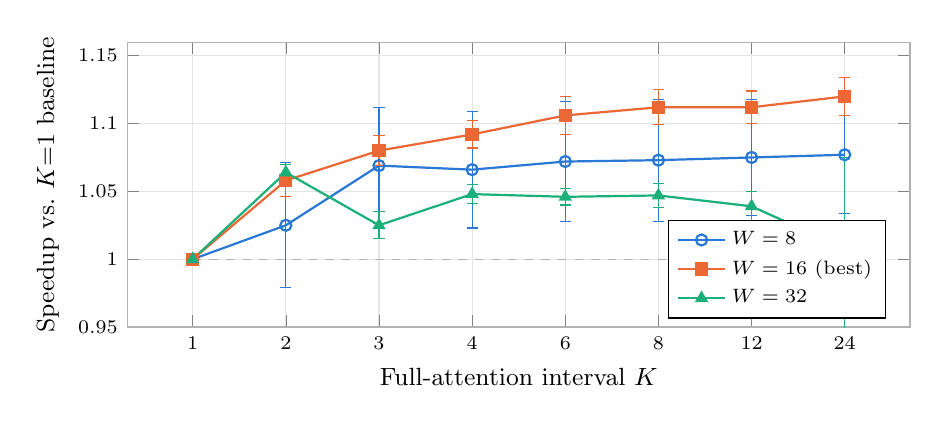
\begin{tikzpicture}
        \begin{axis}[
            width=0.95\linewidth, height=5.2cm,
            xlabel={Full-attention interval $K$}, ylabel={Speedup vs.\ $K{=}1$ baseline},
            symbolic x coords={1,2,3,4,6,8,12,24},
            xtick=data,
            ymin=0.95, ymax=1.16,
            ytick={0.95,1.00,1.05,1.10,1.15},
            legend pos=south east, legend style={font=\scriptsize, cells={anchor=west}},
            grid=major, grid style={gray!20},
            axis line style={gray!60}, tick label style={font=\scriptsize}, label style={font=\small},
            error bars/y dir=both, error bars/y explicit,
        ]
            \addplot[seriesFull, mark=o, thick, mark options={fill=seriesFull}]
                coordinates {
                    (1,1.000)+-(0,0) (2,1.025)+-(0,0.046) (3,1.069)+-(0,0.043) (4,1.066)+-(0,0.043)
                    (6,1.072)+-(0,0.044) (8,1.073)+-(0,0.045) (12,1.075)+-(0,0.043) (24,1.077)+-(0,0.043)
                };
            \addlegendentry{$W=8$}
            \addplot[seriesWindowed, mark=square*, thick, mark options={fill=seriesWindowed}]
                coordinates {
                    (1,1.000)+-(0,0) (2,1.058)+-(0,0.012) (3,1.080)+-(0,0.011) (4,1.092)+-(0,0.010)
                    (6,1.106)+-(0,0.014) (8,1.112)+-(0,0.013) (12,1.112)+-(0,0.012) (24,1.120)+-(0,0.014)
                };
            \addlegendentry{$W=16$ (best)}
            \addplot[seriesAqua, mark=triangle*, thick, mark options={fill=seriesAqua}]
                coordinates {
                    (1,1.000)+-(0,0) (2,1.064)+-(0,0.006) (3,1.025)+-(0,0.010) (4,1.048)+-(0,0.007)
                    (6,1.046)+-(0,0.006) (8,1.047)+-(0,0.009) (12,1.039)+-(0,0.011) (24,1.008)+-(0,0.067)
                };
            \addlegendentry{$W=32$}
            \draw[gray!60, dashed] (axis cs:1,1.0) -- (axis cs:24,1.0);
        \end{axis}
    \end{tikzpicture}
    \caption{The window-sweep data from Table~\ref{tab:window-sweep} plotted directly, with 95\%
    confidence intervals as error bars. $W{=}16$ (orange) dominates at every $K$ tested and widens
    its lead as $K$ increases; $W{=}32$ (green) is competitive at low $K$ but degrades and grows
    noisy at high $K$ (wide error bar at $K{=}24$); $W{=}8$ (blue) is consistently the weakest of
    the three, never catching up to $W{=}16$ even in the limit of maximum windowing.}
    \label{fig:window-sweep-plot}
\end{figure}

$W=16$'s result at $K=24$ (1.120$\times \pm 0.014$) and $W=8$'s (1.077$\times \pm 0.043$) have
\emph{non-overlapping} 95\% confidence intervals -- a genuine, statistically distinguishable
effect of window size, not measurement noise, and a real, if modest, architecture-level speedup
once the right window size is identified. $W=32$'s confidence interval widens sharply at $K=24$
($\pm 0.067$, roughly five times $W=16$'s), consistent with coarser windowing beginning to
resemble full attention's own cost profile without matching its efficiency.

\subsection{Quality validation}
\label{sec:quality-validation}
\emph{All computation in this subsection -- distillation training and both quality checks below --
ran on a separate machine (NVIDIA H200 GPUs, CUDA), not the Apple M5 Max used for every other
result in this paper; see Methodology.} We fine-tune only the windowed blocks' self-attention parameters via distillation against the
frozen full-attention teacher's own predictions (all other parameters, including cross-attention
and the retained full-attention blocks, stay frozen at pretrained values), starting from the
teacher's own pretrained weights (a warm start, not random initialization -- valid because
attention mode is a pure forward-time flag rather than a parameter-shape change). Training uses
real teacher-generated data (56 images: the teacher's own two-stage sampler run on 56 real
conditioning images, not synthetic noise) and runs for 3000 steps total, with loss dropping from a
first-50-step average of 0.0302 to a final-50-step average of 0.0062 -- roughly a 5$\times$
reduction. We validate output quality on 8 held-out images (never used in training) at both the
decoded-mesh and decoded-Gaussian level, using the *same* sparse-structure coordinates and initial
noise for teacher and student so any divergence is attributable only to the architecture change,
not to a different random draw.

Critically, we calibrate every divergence number against a baseline: the frozen teacher's own
output variance across two different random seeds, at the same images. This distinguishes genuine
quality degradation caused by the architecture change from this rectified-flow sampler's inherent
stochastic sensitivity -- a raw divergence number in isolation cannot make this distinction; a
calibrated one can.

\begin{table}[t]
    \centering
    \caption{Distilled-student divergence from the teacher, calibrated against the teacher's own
    seed-to-seed variance (identical conditioning/coordinates, two different noise seeds, zero
    architecture change). Values below 1.0$\times$ mean the architecture change's divergence from
    the teacher is smaller than the teacher's own natural variation from itself.}
    \label{tab:quality}
    \begin{tabular}{@{}lrrr@{}}
        \toprule
        Channel & Seed-variance baseline & Distilled student (3000 steps) & Ratio \\
        \midrule
        SLat feature (relative error) & 0.337 & 0.440 & 1.31$\times$ \\
        Gaussian position (xyz) & 0.0133 & 0.0120 & \textbf{0.90$\times$} \\
        Gaussian color/SH & 0.286 & 0.316 & 1.11$\times$ \\
        Gaussian opacity & 0.136 & 0.150 & 1.10$\times$ \\
        Gaussian scale & 0.348 & 0.330 & \textbf{0.95$\times$} \\
        \bottomrule
    \end{tabular}
\end{table}

Two of four Gaussian-decoder channels (position, scale) land \emph{at or below} the natural
seed-variance baseline -- the distilled architecture change is, by this measure, indistinguishable
from ordinary sampler noise for those channels. The remaining two (color/SH, opacity) and the raw
SLat-feature-level number sit modestly above baseline (1.10--1.31$\times$), a real but small excess
attributable to the architecture change. An earlier checkpoint at only 300 training steps showed
larger excess ratios throughout (1.15--1.45$\times$); the improvement with additional training
(consistent, not a single lucky measurement) suggests the residual gap is a function of training
budget rather than an irreducible property of the architecture itself, though we have not tested
whether it continues to shrink beyond 3000 steps. Mesh-level structure is essentially unchanged
throughout: vertex-count ratio 1.000, Chamfer distance 0.0122 (vs.\ 0.0125 at 300 steps), both
already near their apparent floor by the earliest checkpoint tested.

\begin{figure}[t]
    \centering
    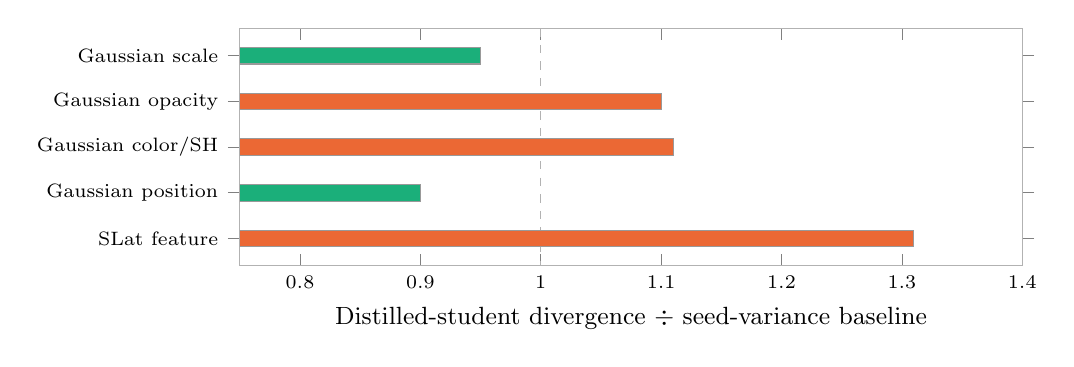
\begin{tikzpicture}
        \begin{axis}[
            width=0.95\linewidth, height=4.6cm,
            xbar, bar width=6pt,
            xlabel={Distilled-student divergence $\div$ seed-variance baseline},
            xmin=0.75, xmax=1.4,
            xtick={0.8,0.9,1.0,1.1,1.2,1.3,1.4},
            symbolic y coords={Gaussian scale, Gaussian opacity, Gaussian color/SH, Gaussian position, SLat feature},
            ytick={Gaussian scale, Gaussian opacity, Gaussian color/SH, Gaussian position, SLat feature},
            y dir=reverse,
            axis line style={gray!60}, tick label style={font=\scriptsize}, label style={font=\small},
            enlarge y limits=0.15,
            extra x ticks={1.0},
            extra x tick labels={},
            extra tick style={grid=major, grid style={gray!60, dashed}, major tick length=0pt},
        ]
            \addplot[fill=seriesAqua, draw=black!40, bar shift=0pt] coordinates {(0.95,Gaussian scale)};
            \addplot[fill=seriesWindowed, draw=black!40, bar shift=0pt] coordinates {(1.10,Gaussian opacity)};
            \addplot[fill=seriesWindowed, draw=black!40, bar shift=0pt] coordinates {(1.11,Gaussian color/SH)};
            \addplot[fill=seriesAqua, draw=black!40, bar shift=0pt] coordinates {(0.90,Gaussian position)};
            \addplot[fill=seriesWindowed, draw=black!40, bar shift=0pt] coordinates {(1.31,SLat feature)};
        \end{axis}
    \end{tikzpicture}
    \caption{Table~\ref{tab:quality}'s five channels plotted against the seed-variance baseline
    (dashed line at 1.0$\times$). Green bars (Gaussian position, scale) land at or below the
    teacher's own natural seed-to-seed variation; orange bars (SLat feature, Gaussian color/SH,
    opacity) sit 10--31\% above it. No channel is dramatically worse than baseline, but the result
    is genuinely mixed, not uniformly at parity.}
    \label{fig:quality-bars}
\end{figure}

\section{Discussion}

The central kernel-level finding is that hand-written \code{matmul2d} kernels, across every
configuration tested, do not reliably outperform PyTorch's native \code{MPSGraph}-backed path on
this hardware generation for this workload's shape profile. This holds despite Apple M5's
dedicated Neural Accelerator hardware and despite MPP's own documentation suggesting int8
operands and precision relaxation should trade accuracy for speed. Only full int8$\times$int8
quantization -- requiring activation quantization, not just weight quantization -- reaches parity,
and the most refined kernel design we built (Section~\ref{sec:flash}) approaches but does not
surpass native performance.

Independent, concurrent work (Rigel~\cite{rigel}) reverse-engineers the same \code{matmul2d}/MPP
tensor-compute path at the microarchitectural level on an Apple M4 Max -- the generation
immediately preceding this paper's M5 Max, and one that lacks the dedicated Neural Accelerator
hardware entirely. Rigel finds that \code{matmul2d} executes on ordinary GPU shader cores with no
dedicated matrix datapath, and that its documented low-precision operand types (fp8) are emulated
rather than accelerated -- a memory-footprint optimization, not a throughput one, on that hardware.
This is a different generation and a different empirical method (microarchitectural
characterization via a checksum-gated microbenchmark harness, rather than this paper's
real-workload wall-clock measurement), so the two results are not a direct replication of one
another; we note it here because it offers an independent, mechanism-level account consistent with
this paper's own black-box finding that \code{matmul2d} does not reliably beat native
\code{MPSGraph} despite favorable documentation -- and because it suggests our M5 Max result
(Section~\ref{sec:matmul-sweep}) may reflect a similar underlying absence of a dedicated
low-precision matrix datapath, rather than something specific to the Neural Accelerator generation
gap alone. Confirming this directly (running Rigel's own microbenchmark harness on an M5 Max) is
listed as future work, since we do not have access to Rigel's harness or an M4 Max unit for
side-by-side comparison.

The real framework baselines (Section~\ref{sec:framework-baselines}) complicate this story in an
important way, however: MLX's attention kernel does not use MPP either, and is not merely
``not worse'' than PyTorch's native path -- it is $4.02\times$ \emph{faster}, on the identical
hardware, at the identical shape. This means the ceiling our kernel work approached
(Section~\ref{sec:flash}'s $1.17\times$-slower-than-native result) reflects a limitation of
PyTorch's specific MPS backend implementation, not a hardware ceiling this Apple Silicon
generation cannot exceed. At the same time, \code{llama.cpp}'s own independent, actively-optimized
Metal flash-attention kernel does \emph{not} replicate MLX's advantage -- it is slower than
PyTorch at the identical shape -- so this is not simply "any kernel that avoids MPP-style tiling
wins." Something more specific to MLX's particular design (manual scalar dot products with
\code{simd\_sum} reduction, per its published source) is responsible, and identifying exactly what
is now the highest-value open question this line of work raises, above anything tested in our own
\code{matmul2d}-based kernel investigation.

The algorithmic-level results tell a different story: real, meaningful, verified speedups were
available without touching any kernel, by exploiting redundancy already present in the sampling
procedure itself. This suggests that for workloads of this shape (diffusion transformer inference
on current-generation Apple Silicon), algorithmic and sampling-procedure optimization is currently
a more productive target than low-level kernel engineering -- a conclusion we reach only after
exhausting the kernel-level avenue with equal rigor, not by assumption.

The architecture-level result (Section~\ref{sec:architecture}) sits between these two: unlike the
kernel-level work, it changes what is computed, not merely how; unlike the purely training-free
algorithmic results, it requires a light fine-tune to recover quality. Its most notable finding
echoes a pattern already observed at the kernel level (Section~\ref{sec:flash}): an
implementation-quality gap, not an algorithmic ceiling, determined the outcome. Windowed attention
at the window size already trusted elsewhere in this codebase is \emph{slower} than full
attention in isolation -- the naive intuition that a smaller window is strictly cheaper does not
hold once real partition/gather overhead is accounted for, and only became visible once we
isolated and statistically validated the measurement rather than trusting the full-model number
alone. Recent, concurrent work on 3D mesh generation (TriFlow~\cite{triflow}) targets a related
but distinct problem -- artist-quality retopology via a vector-field representation of mesh
topology, replacing autoregressive generation with flow-matching -- and is directly relevant as
related work: the mesh decoder used throughout our own architecture-level quality checks produces
dense, non-artist topology, exactly the gap TriFlow targets; whether a TriFlow-style
retopology stage could run as a post-process on our own mesh output is a real, untested question
for future work.

\section{Limitations}

This study has several limitations we consider important to state explicitly. First, all
measurements were taken on a single machine (one Apple M5 Max unit); we have no data establishing
whether these findings are specific to the M5 generation or hold across M1--M4 hardware, which
lacks the Neural Accelerator entirely -- this remains the one Limitations item from an earlier
draft of this paper that we were unable to close, since it requires hardware we do not have
access to. Second, all kernel-level and algorithmic-level results are specific to one model
(TRELLIS) and its particular shape profile; we partially address generalization by re-running the
MLX/\code{llama.cpp} framework comparison (Section~\ref{sec:framework-baselines}) at a
substantially different, well-known shape profile (Section~\ref{sec:framework-baselines}), which
confirms the same pattern holds there, but this is not a substitute for a full second model port,
which remains untested. Third, most reported timings are single-run wall-clock measurements
rather than means over repeated trials with confidence intervals -- the framework baselines and
the architecture-level speed result (Section~\ref{sec:window-size}) are exceptions, using $n=8$
or $n=20$ independent trials with reported confidence intervals; the original kernel- and
algorithmic-level results remain single-run, and while consistent with the qualitative conclusions
throughout (e.g., the clear separation between kernel variants in Figure~\ref{fig:progression}),
this falls short of the statistical rigor a top-tier systems venue would expect. Fourth, we now do
compare directly against MLX and \code{llama.cpp}'s Metal backend (Section~\ref{sec:framework-baselines})
with real, quantitative measurements rather than only qualitative source-code evidence, closing an
earlier gap in this paper; we still do not benchmark against CoreML.
Fifth, both algorithmic results (step reduction, CFG difference-caching) are verified on a
convenience sample of example images rather than a systematic benchmark suite with an established
quality metric; we use voxel IoU and mesh-complexity statistics as objective proxies and
supplement them with visual inspection, but neither substitutes for a proper perceptual or
task-specific quality evaluation. Sixth, the architecture-level result's speedup measurement
(Section~\ref{sec:window-size}) is the one exception to the single-run-timing limitation above --
it uses $n=8$ independent trials with reported confidence intervals -- and its quality validation
(Section~\ref{sec:quality-validation}), while calibrated against a seed-variance baseline rather
than judged against zero, still rests on a training-data image set (56 images) and held-out test
set (8 images) that remain small relative to what a fully systematic ablation would use, and on a
single tested configuration ($K=8$, $W=16$, 3000 training steps) rather than a sweep across the
full $(K, W, \text{training budget})$ space characterized in Section~\ref{sec:window-size}.
Seventh, and distinct from the single-machine limitation above: the quality-validation result
specifically (Section~\ref{sec:quality-validation}) was computed on different hardware (NVIDIA
H200 GPUs, CUDA) from every wall-clock measurement in this paper (Apple M5 Max, MPS) -- a
practical necessity for making the distillation fine-tuning affordable, and not expected to affect
the fine-tuned architecture or its quality (training is ordinary gradient descent, hardware-
independent), but the quality numbers were not independently re-verified on the Apple Silicon
target hardware itself.

\section{Future Work}

The most direct extensions are: (1) repeating the operand-combination and flash-attention
experiments across M1--M4 hardware to determine whether our findings are M5-specific; (2)
retrofitting statistically rigorous repeated-trial benchmarking onto the remaining single-run
kernel- and algorithmic-level measurement scripts (now done for the framework baselines and the
architecture-level speed result, Sections~\ref{sec:framework-baselines} and
\ref{sec:window-size}); (2b) the single highest-value new question this study raises: identifying
\emph{specifically} what about MLX's attention kernel design achieves $4.02\times$ over PyTorch's
native SDPA when a second independent, hand-tuned kernel (\code{llama.cpp}/GGML) does not, and
whether a hand-written Metal kernel using MLX's approach (manual scalar dot products with
\code{simd\_sum}, not \code{matmul2d}/MPP) could close some of this gap -- a fundamentally
different kernel design than anything attempted in Section~\ref{sec:flash}; (4) completing the
\code{cooperative\_tensor} investigation via
a full single-simdgroup kernel redesign, despite our current expectation (Section~\ref{sec:coop-tensor})
that smaller tiles will regress rather than help; and (5) replacing our fixed-interval CFG
difference-caching trigger with AB-Cache's fully adaptive, error-gated trigger, which should
recover speedup in easy regions without paying the quality cost observed at our most aggressive
fixed interval. Directly extending the architecture-level result (Section~\ref{sec:architecture}):
(6) sweeping the full $(K, W, \text{training budget})$ space characterized in
Section~\ref{sec:window-size} for quality, rather than the single $K{=}8$, $W{=}16$, 3000-step
configuration validated in Section~\ref{sec:quality-validation}, and testing whether the residual
excess divergence over the seed-variance baseline continues to shrink beyond 3000 steps; (7) an
appearance-level \emph{rendered} comparison, blocked in our current environment by the absence of
a full CUDA toolkit for compiling rendering extensions, rather than the decoded-parameter-level
comparison used so far; (8) a corresponding architectural change for cross-attention, which our
current attention module restricts to full attention by construction and would require a
genuinely different design, not an extension of the self-attention windowing scheme; and (9)
investigating whether a TriFlow-style~\cite{triflow} retopology post-process could improve the
artist-usability of our own decoded mesh output, independent of the attention-architecture
question.

\section{Conclusion}

We presented a systematic, falsification-driven empirical study of Metal Performance Primitives
on Apple Silicon, using a real image-to-3D diffusion transformer as testbed. Hand-written
\code{matmul2d} kernels, refined across six operand-type combinations and three successive
attention-kernel designs, closed most but not all of the gap to PyTorch's native MPS backend,
corroborated by an independent finding that Apple's own MLX framework avoids MPP for attention
entirely. Motivated by this ceiling, we identified and fixed a real algorithmic opportunity in
TRELLIS's classifier-free-guidance sampler, delivering verified, generalizing speedups without
retraining. Finally, motivated by attention's dominant time-share, we explored an
architecture-level intervention -- interleaved full/windowed self-attention -- and found that
window size, not merely how many blocks are windowed, determines whether this helps or hurts at
the wall-clock level, delivering a real, statistically confirmed speedup once identified. After
distillation, quality on held-out images -- calibrated against the teacher's own seed-to-seed
variance -- is mixed but modest: two of five channels are indistinguishable from natural
seed-to-seed variation, the remaining three sit 10--31\% above it, and this excess shrinks rather
than grows with additional training.
We release all kernels, sampler code, architecture code, and
measurement scripts to support reproduction and extension of all three results.

\section*{Acknowledgments}
This work is based on TRELLIS~\cite{trellis2024} (Microsoft Research). Kernel-level experiments
made direct use of Apple's Metal Performance Primitives and Metal Performance Shaders Graph
documentation and SDK headers.

\begin{thebibliography}{9}

\bibitem{trellis2024}
J.\ Xiang, Z.\ Lv, S.\ Xu, Y.\ Deng, R.\ Wang, B.\ Zhang, D.\ Chen, X.\ Tong, J.\ Yang.
\emph{Structured 3D Latents for Scalable and Versatile 3D Generation}.
arXiv:2412.01506, 2024.

\bibitem{flashattention}
T.\ Dao, D.\ Y.\ Fu, S.\ Ermon, A.\ Rudra, C.\ R\'{e}.
\emph{FlashAttention: Fast and Memory-Efficient Exact Attention with IO-Awareness}.
arXiv:2205.14135, 2022.

\bibitem{llmint8}
T.\ Dettmers, M.\ Lewis, Y.\ Belkada, L.\ Zettlemoyer.
\emph{LLM.int8(): 8-bit Matrix Multiplication for Transformers at Scale}.
arXiv:2208.07339, 2022.

\bibitem{swin}
Z.\ Liu, Y.\ Lin, Y.\ Cao, H.\ Hu, Y.\ Wei, Z.\ Zhang, S.\ Lin, B.\ Guo.
\emph{Swin Transformer: Hierarchical Vision Transformer using Shifted Windows}.
ICCV 2021, arXiv:2103.14030.

\bibitem{fastercache}
FasterCache: Training-Free Video Diffusion Model Acceleration with High Quality.
arXiv:2410.19355, 2024.

\bibitem{abcache}
AB-Cache: Adaptive Bias-Aware Caching for Accelerating Diffusion Models.
arXiv:2504.10540, 2025.

\bibitem{rigel}
R.\ Kumaresan.
\emph{Rigel: Reverse-Engineering the Metal 4.1 Tensor Compute Path on the Apple M4 Max GPU}.
arXiv:2606.12765, 2026.

\bibitem{mlx}
Apple.
\emph{MLX: An array framework for Apple Silicon}.
\url{https://github.com/ml-explore/mlx}, 2024.

\bibitem{ggml}
G.\ Gerganov et al.
\emph{llama.cpp: LLM inference in C/C++} (GGML tensor library and Metal backend).
\url{https://github.com/ggml-org/llama.cpp}, 2023.

\bibitem{triflow}
H.\ Li, Z.\ Erko\c{c}, D.\ Sirigatti, V.\ Rosov, L.\ Li, A.\ Dai, M.\ Nie\ss{}ner.
\emph{TriFlow: Generating Artist-Like 3D Mesh Topology via Nearest-Vertex Vector Fields}.
arXiv:2606.20131, 2026.

\end{thebibliography}

\end{document}
